\chapter{Results}\label{ch:results}
In this chapter, we will mainly present the results obtained on our dataset by following the methodology previously discussed. Before doing so, however, we feel like a brief discussion on quality evaluation of word embeddings is necessary.

\section{Evaluation of word embeddings}
Techniques such as word2vec are powerful tools for representing meaning using geometry. As with any model working on real data, it is important to conduct a rigorous evaluation which can justify its goodness. Our scenario makes no exception, especially given the exploratory nature of the task we are after. Relying so much on this model to explore the dataset while looking for meaningful semantic relationships means we must be sure that the model actually learned these relationships.

Good overviews of evaluation methods for word embeddings can be found in \cite{schnabel2015evaluation} and \cite{bakarov2018survey}. The reason why there exist many evaluation methods can be reconduced to the instrinsic difficulty in determining semantic similarity/relatedness in a broader sense. If we add to that that words have multiple degrees of similarity, that the structure of embeddings can greatly vary across corpora and models, and that, in general, there is a lack of correlation between different performance scores, the challenges of choosing or designing a meaningful evaluation system become even more evident. 

There are two evaluation methods we find to be the most suitable here. The first is based on \emph{Gold Standard Corpora} (\acsfont{GSC}), lists compiled by hand by linguists or field experts where pairs of words are given an explicit similarity score. These lists are then compared with the model, and an aggregated estimate is calculated (usually, Pearson or Spearman correlation coefficient). Such an estimate reports the similarity of semantic relationships as inferred by the embedding to the semantic relationships as inferred by human experts. The advantage of adopting \acsfont{GSC} is that they can be compiled to be quite domain-specific; specificity is useful to disambiguate, for example, cases of polysemy (words with more than one meaning) and in general helps to restrict semantic judgments to the domain the model is supposed to work in\footnote{For example, \cite{sugathadasa2017synergistic} demonstrated the usefulness of using domain-specific \acsfont{GSC} to evaluate embeddings trained on legal documents.}. 

We are working in the music domain; for this reason, we looked for openly available \acsfont{GSC} to evaluate our model, without success. Unfortunately, as \cite{wissler2014gold} observe, building a \acsfont{GSC} manually results in a costly process, both in terms of time and resources. This prevented us from creating our own evaluation corpus here, but we hope this gap can be filled as soon as possible.

The second evaluation method taken into consideration is somehow similar to the one just discussed, with two main differences:
\begin{enumerate}
\item the lists are not domain-specific, but can span rather general contexts;
\item the lists are based on judgments of people who do not necessarily have a background in Linguistics.
\end{enumerate}
The advantage of using such lists over \acsfont{GSC} is that the former are more widely available. The drawback is that, when comparing their content with domain-specific datasets such as ours, the model's goodness can suffer from being tested on words not belonging or marginal to that specific context.

\subsection{Evaluating our model}\label{subsec:eval}
What has been described in the last paragraph is exactly what happened to us. We decided to adopt a standard list, the \emph{wordsim353}\footnote{Introduced in \cite{finkelstein2001placing} and available at \url{http://alfonseca.org/eng/research/wordsim353.html}}, and we tested our embedding with it. The aggregated estimate yielded a Spearman's rank correlation coefficient of 0.45 ($p$ $<$ 0.05). However, almost 60\% of the tuples in the list could not be evaluated, because they featured terms which did not appear at all in our corpus.

Previous results thus demand other ways of assessing the quality of our embedding. Having to deal with music, we proceeded with more empirical explorations of the model, looking for meaningful musical semantic relationships. Taking inspiration from \cite{mikolov2013distributed}, where the authors observed how their model could implicitly learn and organize concepts such as countries and capitals and their association, we explored whether our embedding could discriminate between \emph{musicians} and their relative \emph{instruments}.

\autoref{fig:player-instr} shows the result of this exploration. It is interesting to observe not only how the model learned to discriminate between the concept of musician and the concept of musical instrument, but also how it almost mantained the same hierarchy between musicians and instruments (except for the drummer-drums pair). Terms traditionally associated with rock-type of genres appear towards the bottom, whereas moving towards the top part of the plot more classic instruments/musicians appear. The voice-singer pair appears in a more distant corner, likely due to the polysemous nature of the term \emph{voice} and to the fact that voice cannot be properly defined as an instrument.

\begin{figure}[bth]
	\myfloatalign
	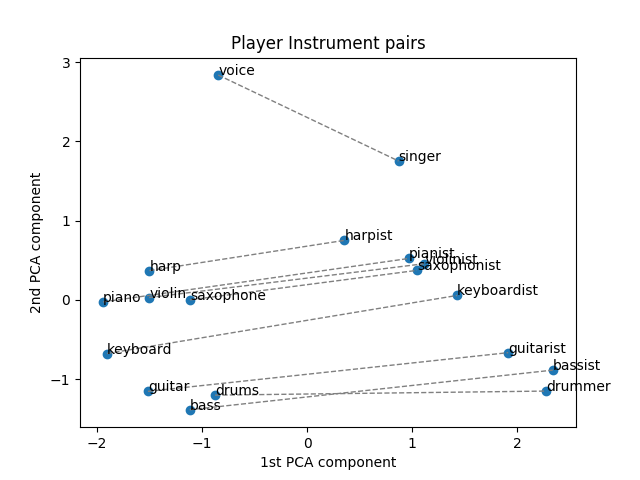
\includegraphics[width=\linewidth]{gfx/player-instrument2}
	\caption[\acsfont{PCA} plot of player-instrument word pairs]{Plot of a \acsfont{PCA} with 2 components performed on word vectors for pairs of musicians-played instrument. The model has succesfully learned the difference between these two classes of musical concepts (instruments on the left, musicians on the right).}
	\label{fig:player-instr}
\end{figure}

Next, we briefly explored how the model organized music genres. A \acsfont{PCA} plot of a list of music genres words is shown in \autoref{fig:genres}. What the model seems to have learned is interesting. On the far left-side of the graph we find more rhythm-driven genres (rap, hip-hop, dance, techno, house), while all the genres towards the bottom seem to have in common their black origins. Classical music, opera and religious appear on the top-right, while rock, metal, pop and alternative live towards the center of the plot. On the far right-side are featured typical traditional American genres, such as bluegrass, folk, country, gospel and blues.

\begin{figure}[tp]
	\myfloatalign
	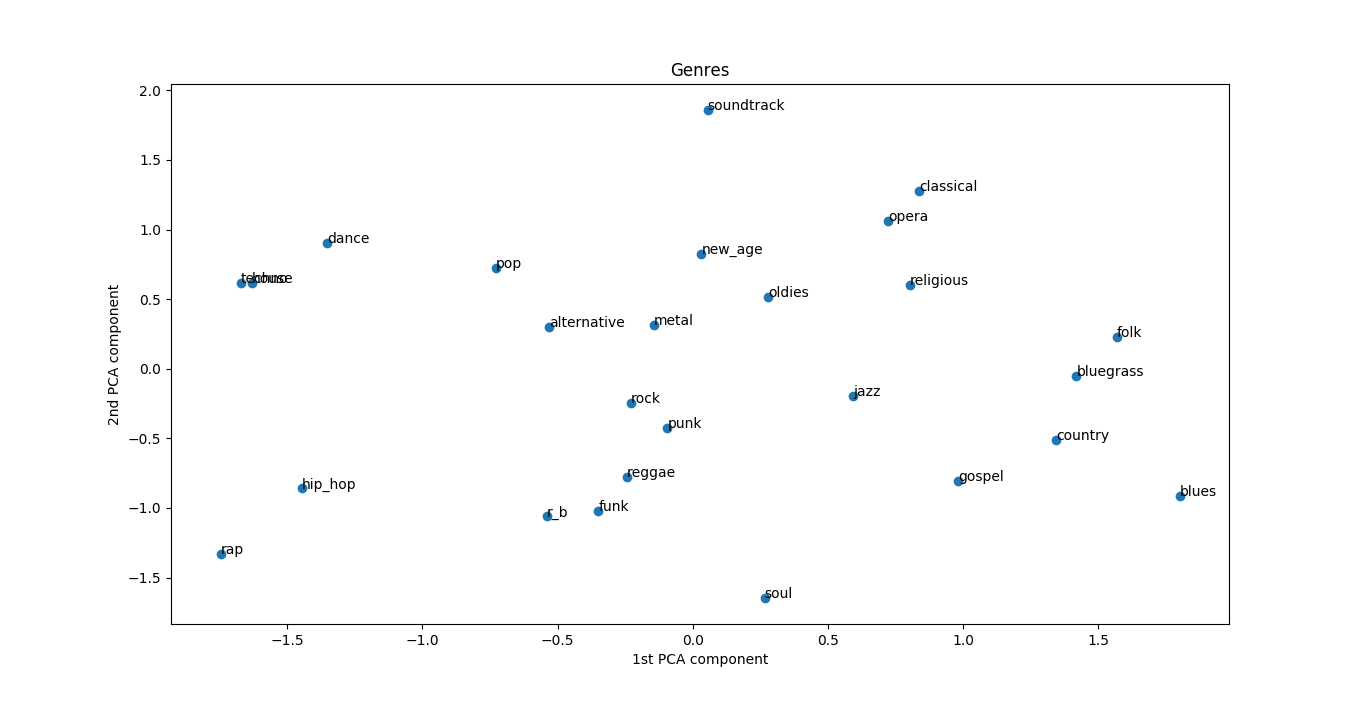
\includegraphics[angle=-90,origin=c,width=\linewidth]{gfx/genres}
	\caption[\acsfont{PCA} plot of music genres words]{Plot of a \acsfont{PCA} with 2 components performed on word vectors for music genres.}
	\label{fig:genres}
\end{figure}

These are just two examples of some empirical observations we made on our dataset regarding musical concepts. While it is true that no rigorous evaluation confirmed how reliable the model effectively is, the plots shown above give us enough confidence that the model can represent music-related concepts with a reasonable degree of semantic organization. For sure, when more proper evaluation techniques will be avaliable for this type of data, it will be advisable for us to provide a more grounded justification of our embedding.

\section{Results}
\subsection{Nearest neighbours}\label{subsec:nearest}
For each of the aesthetic terms listed in \autoref{sec:query}, we first queried our model for the 10 words which appeared closer to the input, in terms of cosine similarity between their vector representations. 

The 10 closest words returned by the model for the words \emph{beauty--beautiful--beautifully} are reported in \autoref{tab:beauty10nearest}. The first interesting result is that for \emph{beauty} and \emph{beautifully}, all of the top 10 nearest words are nouns and adverbs, respectively, just like the query words, whereas for \emph{beautiful} not only adjectives are retrieved, but also some adverbs (\emph{achingly} and \emph{crushingly}). For all of three words, there is no term living notably close to the respective query word (if this was the case, there would be semantic equivalence), since all of the cosine similarities are below 0.7. Third, there are very few words referring to concrete objects or qualities; abstract concepts seem to be dominant.

\begin{table}[tbh]
\myfloatalign
\small
\begin{tabular}{ll}
\toprule
\multicolumn{2}{c}{beauty}\\ \midrule
	ugliness & 0.6402 \\
	serenity & 0.6355 \\
	loveliness & 0.6252 \\
	listlessness & 0.6197 \\
	sublimity & 0.6191 \\
	prettiness & 0.6159 \\
	quietude & 0.6155 \\
	fragility & 0.6143 \\
	elegance & 0.6049 \\
	imperfection & 0.5943 \\
	\bottomrule
\end{tabular}
\begin{tabular}{ll}
\toprule
\multicolumn{2}{c}{beautiful}\\ \midrule
	gorgeous & 0.6994 \\
	lovely & 0.6354 \\
	transfixing & 0.623 \\
	achingly & 0.6195 \\
	wonderful & 0.6195 \\
	crushingly & 0.6173 \\
	stunning & 0.6089 \\
	affecting & 0.6042 \\
	spellbinding & 0.6042 \\
	beguiling & 0.602 \\
	\bottomrule
\end{tabular}
\begin{tabular}{ll}
\toprule
\multicolumn{2}{c}{beautifully}\\ \midrule
	exquisitely & 0.6669 \\
	gorgeously & 0.6542 \\
	sumptuously & 0.6523\\ 
	flawlessly & 0.6452\\
	pristinely & 0.6288\\
	thoughtfully & 0.6242\\
	marvelously & 0.6166\\
	impeccably & 0.6144 \\
	elegantly & 0.6124\\
	superbly & 0.5948\\
\bottomrule
\end{tabular}
\caption[Nearest neighbours for \emph{beauty-beautiful-beautifully}]{Top 10 nearest neighbours for the words \emph{beauty--beautiful--beautifully}. Left column reports the word, right column the cosine similarity.}
\label{tab:beauty10nearest}
\end{table}

\autoref{tab:aesth10nearest} reports the 10 closest words returned by the model for the words \emph{aesthetic--aesthetics}. It is more challenging to give an interpretation of the semantic relationships in these results. \emph{Aesthetics} appears to be associated to concepts bound to tradition, universalism and timelessness, conveying images of something that is there and should not be questioned (\emph{tenets}; \emph{paradigms}; \emph{conversant}; \emph{vocabularies}; \emph{idioms}; \emph{forbears}). This idea partly returns for \emph{aesthetic}, but here the concepts seem to have a more abstract acception, which can be subject to personal attitude and interpretation (\emph{worldview}; \emph{ethos}; \emph{principles}; \emph{approach}).

\begin{table}[bth]
\myfloatalign
\small
\begin{tabular}{ll}
\toprule
\multicolumn{2}{c}{aesthetic}\\ \midrule
worldview & 0.5978\\
purview & 0.5902\\
aesthetics & 0.5875\\
ethos & 0.5819\\
principles & 0.5768\\
approach & 0.5758\\
alchemical & 0.5756\\
plasticity & 0.5729\\
perfectionism & 0.5672\\
frameworks & 0.5664\\
\bottomrule
\end{tabular}
\begin{tabular}{ll}
\toprule
\multicolumn{2}{c}{aesthetics}\\ \midrule
tenets & 0.6536\\
affinities & 0.653\\
paradigms & 0.652\\
synthesists & 0.6382\\
conversant & 0.6332\\
bastardizing & 0.633\\
vocabularies & 0.6316\\
idioms & 0.6286\\
hybridization & 0.6231\\
forbears & 0.6219\\
\bottomrule
\end{tabular}
\caption[Nearest neighbours for \emph{aesthetic-aesthetics}]{Top 10 nearest neighbours for the words \emph{aesthetic--aesthetics}.}
\label{tab:aesth10nearest}
\end{table}

Finally, in \autoref{tab:ugly10nearest} the resulting nearest neighbours for \emph{ugliness--ugly} have been reported. \emph{Ugliness}, up to now, is the only term whose cosine similarities with retrieved neighbours are almost all above 0.7. It is interesting to observe how words close to it do not necessarily possess a negative connotation (\emph{placidity}; \emph{exhilaration}; \emph{surreality}). The same cannot be said for \emph{ugly}: almost the totality of its neighbours have a very negative polarity, except for the first two (\emph{casanova}; \emph{ugly})\footnote{This very last observation is easily explained: \emph{Ugly Casanova} and \emph{Ugly Duckling} are the names of two bands.}.

\begin{table}[bth]
\myfloatalign
\small
\begin{tabular}{ll}
\toprule
\multicolumn{2}{c}{ugliness}\\ \midrule
placidity & 0.7308\\
messiness & 0.7307\\
discord & 0.7254\\
exhilaration & 0.7229\\
surreality & 0.71\\
discomfort & 0.7088\\
nakedness & 0.701\\
listlessness & 0.7005\\
eeriness & 0.6969\\
bleakness & 0.695\\
\bottomrule
\end{tabular}
\begin{tabular}{ll}
\toprule
\multicolumn{2}{c}{ugly}\\ \midrule
casanova & 0.6006 \\
duckling & 0.5876\\
angry & 0.5732\\
vulgar & 0.5352\\
inappropriately & 0.5347\\
unrelentingly & 0.5328\\
repellant & 0.5265\\
unrepentantly & 0.5259\\
disgusting & 0.5222\\
exasperating & 0.5201\\
\bottomrule
\end{tabular}
\caption[Nearest neighbours for \emph{ugly-ugliness}]{Top 10 nearest neighbours for the words \emph{ugly--ugliness}.}
\label{tab:ugly10nearest}
\end{table}

\subsection{Clustering}
The results presented up to now hint at some patterns in the way our model organizes both musical and aesthetic information. Here we tried to cluster the 100 nearest neighbours to each aesthetic term using a k-means strategy. Since k-means should be provided with the number of clusters the algorithm has to compute (parameter $k$), we ran different analyses varying $k$ and evaluating eacht time the output.

Unfortunately, our quest looking for meaningful word clusters was not particularly successful. Clusters generated in this way look messy, as they include set of words for which finding a common semantic thread is difficult. As an example, we provide the clusters generated for the term \emph{beauty}, with $k$ $=$ 7, in \autoref{tab:clus}. Clusters computed on the other words of our list and with other values for $k$ have been omitted, since they all more or less follow the same pattern -- or, better said, \emph{non}-pattern. 

As we can see, there is a dominating cluster (cluster \#3) containing a big amount of terms which do not appear to have much in common with each other. There are clusters made of only one word, while clusters \#1, \#6 and \#7, which are neither too big or too small, still appear to have been built arbitrarily. Increasing the value of $k$ to try to ``break down'' in more meaningful chunks overly sized clusters, such as cluster \#3 here, has had the only effect of generating a higher number of small clusters containing only one or two words.

\begin{table}[t]
\myfloatalign
\small
\begin{tabularx}{\textwidth}{lX}
\toprule
\acsfont{cluster 1} & prettiness, brightness, delicacy, richness \\
\acsfont{cluster 2} & majesty \\
\acsfont{cluster 3} & listlessness, sublimity, quietude, gorgeousness, gentleness, melancholia, hopefulness, steadiness, discord, undisturbed, eeriness, combustion, peacefulness, bittersweetness, togetherness, coldness, aggressiveness, otherworldliness, pensiveness, nourishment, sakura, placidity, necessities, wrongness, greenery, shroud, insoluble, stateliness, frailty, bleakness, circularity, mutability, solemnity, pleasantness, crispness, clumsiness, ominousness, attains, nakedness, humankind, incompleteness, cultivation, ethereality, disquietingly, solidity, softness, impenetrability, chilliness, unhampered, remoteness, soulfulness, engravings, resourcefulness, jubilance, disquiet, apprehension, manmade, malevolence, splendor, precariousness, enormity, disconnection, wonderment, peril, carnality, trimmings, commotion, vibrancy, engulfing, expansiveness, symbiosis \\
\acsfont{cluster 4} & warmth \\
\acsfont{cluster 5} & sadness \\
\acsfont{cluster 6} & ugliness, serenity, contemplation, elation, exhilaration, vulnerability, pessimism, disorientation, tranquility, uneasiness \\
\acsfont{cluster 7} & loveliness, fragility, elegance, imperfection, poignancy, strangeness, transparency, messiness, lucidity, eloquence, intrigue, persistence \\
\bottomrule
\end{tabularx}
\caption{K-means clustering on the nearest neighbours of the word \emph{beauty}}
\label{tab:clus}
\end{table}

In our opinion, there could be three explanations for this behaviour. First, the model could have failed to learn a meaningful representation of semantic relationships between abstract terminology. Abstractness, in fact, seems to be almost the only thread connecting the reported data. This would in part disprove the observations reported in \autoref{subsec:nearest}. Second, the intrinsic difficulties of defining aesthetic terms could have had the effect of projecting them in corners of the word embedding at the intersection of many different semantic areas. This would make it impossible to find common conjunction points between these areas. Third, the model could simply be overfit on the data. If this was the case, the vector representations of words would almost become like one hot vectors, every one living independently from the others without any connection. This however would disprove many of the things we observed in \autoref{subsec:eval}.

\section{Google News dataset}
Finally, we decided to perform a similar analysis on a different model. This model is not trained on specific music-related data, and was provided by \citeauthor{mikolov2013distributed} as part of their research\footnote{\url{https://drive.google.com/file/d/0B7XkCwpI5KDYNlNUTTlSS21pQmM/}}. The training has been carried out on a dataset of about 100 billion words coming from a huge collection of Google News articles, using a Skip-gram architecture with negative sampling. Generated word vectors have 300 dimensions, while the size of the vocabulary has been cut down by us to the first 500\,000 words, according to their frequency in the corpus (only the most frequent have been kept).

In this scenario, our clustering attempts have proven to be much more successful. We have queried the model for the 500 nearest neighbours\footnote{This number has been chosen instead of 100 for two reasons: \emph{(a)} this dataset is much bigger in size and scope, thus potentially including many more concepts related to beauty other than music; \emph{(b)} the authors did not lowercase the dataset before training, which means that, for example, both \emph{beautiful} and \emph{BEAUTIFUL} are included in the vocabulary.}, and clustered them using k-means. The results for the term \emph{beauty} setting $k$ $=$ 15 are shown in \autoref{tab:gbeauty} (results have been cut down to ten words per cluster). The first thing that jumps to the eye is how much the quality of the clusters improves. All of the clusters contain semantically related words, or words belonging to a common topic. It is also noticeable how much more concrete the concept of beauty appears to be in a general context; many are the references to femininity, sensuality, cosmetics, personal grooming, but also to nature, flowers, architecture. Sadly, not much appears about arts and music.

\begin{table}[tp]
\myfloatalign
\small
\begin{tabularx}{\textwidth}{lX}
\toprule
\multicolumn{2}{c}{beauty} \\
\midrule
\acsfont{cluster 1} & Beauty, skincare, cosmetics, Natural\_Beauty, haircare, Pantene, Shu\_Uemura, Aveda, Lancome, Cosmetics, ... \\
\acsfont{cluster 2} & esthetics, aesthetic, aesthetics, artistry, esthetic, visual\_splendor, artifice, intricacy, originality, starkness, ... \\
\acsfont{cluster 3} & scenic\_beauty, beautiful\_scenery, sweeping\_vistas, breathtakingly\_beautiful, landscapes, splendours, scenery, gorgeous\_scenery, sceneries, picturesque\_scenery, ... \\
\acsfont{cluster 4} & lip\_balms, shampoos\_conditioners, paraben\_free, Body\_Wash, lip\_glosses, aging\_creams, skin\_whitening, shower\_gels, cosmeceuticals, cosmeceutical, ...
 \\
\acsfont{cluster 5} & eyelash\_extensions, estheticians, cosmetic, stylist, hair\_styling, salon, hair\_extensions, esthetician, false\_eyelashes, Makeup, ...\\
\acsfont{cluster 6} & loveliness, magnificence, splendor, serenity, grandeur, majesty, sensual\_pleasures, splendors, sublimity, tranquility, ... \\
\acsfont{cluster 7} & lingerie, Glamour, bridal, fashion, sexy\_lingerie, Allure, beachwear, boho\_chic, StyleList, bridal\_boutique, ... \\
\acsfont{cluster 8} & glamor, gorgeousness, sexiness, pulchritude, fabulousness, classiness, va\_va\_voom, je\_ne\_sais\_quoi, sparkle, tackiness, ... \\
\acsfont{cluster 9} & radiance, naturalness, uniqueness, prettiness, allure, sensuality, timelessness, exoticism, sensuousness, pureness, ... \\
\acsfont{cluster 10} & beauties, plumpness, curvaceous, feminine, curvy, womanly, voluptuous, supermodel, hourglass\_figure, glamorously, ... \\
\acsfont{cluster 11} & PURE\_ranges, fragrance, proto\_col, BEAUTY, perfume, essences, On\_Group.co.uk\_manufacture, handcrafted\_jewelry, floral, Lush, ... \\
\acsfont{cluster 12} & beautiful, gorgeous, ethereal\_beauty, ravishing, sensual, luscious, fabulous, stunningly\_beautiful, sensuous, alluring, ... \\
\acsfont{cluster 13} & elegance, rustic\_charm, timeless\_elegance, opulence, interior\_decor, décor, understated\_elegance, decor, luxe, craftsmanship, ... \\
\acsfont{cluster 14} & spa, spas, aromatherapy, luxurious\_spa, pampering, pamper\_yourself, Aromatherapy, manicure\_pedicure, Spa, Spas, ... \\
\acsfont{cluster 15} & femininity, womanhood, individuality, ordinariness, preciousness, specialness, aliveness, spirituality, wholeness, intimacy, ...\\
\bottomrule
\end{tabularx}
\caption{K-means clustering on the nearest neighbours of the word \emph{beauty} (Google News dataset)}
\label{tab:gbeauty}
\end{table}

As a final point, in \autoref{tab:gbfully} is reported one of the clusters that showed up while exploring the neighbours of \emph{beautifully} in this model. It is evident why it caught our attention: this is the most fulgid example, up to now, of real, tangible musical features that people might be addressing when talking about beauty in music.

\begin{table}
\myfloatalign
\small
\begin{tabularx}{\textwidth}{X}
\toprule
beautifully\_sung, recitatives, vocalism, harmonically, orchestral\_accompaniment, rhythmically, lyricism, rhythmical, melodically, cadenzas, contrapuntal, tonalities, sonority, acoustically, pizzicato, sonorities, Tyagaraja, rhythmic\_patterns, legato, fugues, expressivity \\
\bottomrule
\end{tabularx}
\caption{Cluster extracted from the neighbours of the word \emph{beautifully} (Google dataset)}
\label{tab:gbfully}
\end{table}
